\newpage
\section{Skinning}

\begin{figure}[!htb]
    \centering
    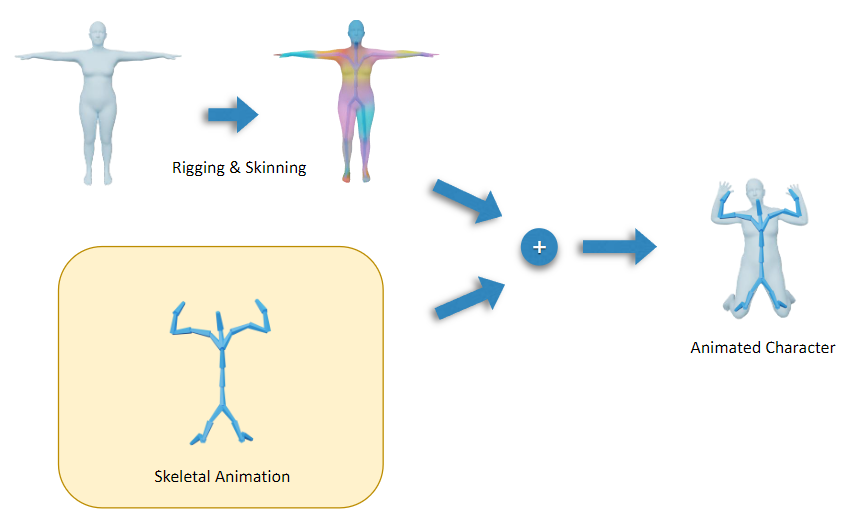
\includegraphics[width=0.618\linewidth]{pic/1057/Character Animation Pipeline}
    \caption{Character Animation Pipeline}
\end{figure}


\begin{itemize}
    \item Rigging: 绑定, 可能会添加额外控制器.
    \item Skinning: 特殊的绑定, 将皮肤绑定到骨骼.
\end{itemize}

Skinning Deformation: 
\begin{align*}
    \bx' &= Q'Q^\top (\bx - \bo) + \bo'\\
    &= Q' \br + \bo'\\
    Q' &= RQ\\
    \bo' &= \bo + \bt\\
    \br &= Q^\top (\bx - \bo)
\end{align*}
$\br$ 表示关节到蒙皮的局部坐标. 

\begin{figure}[!htb]
    \centering
    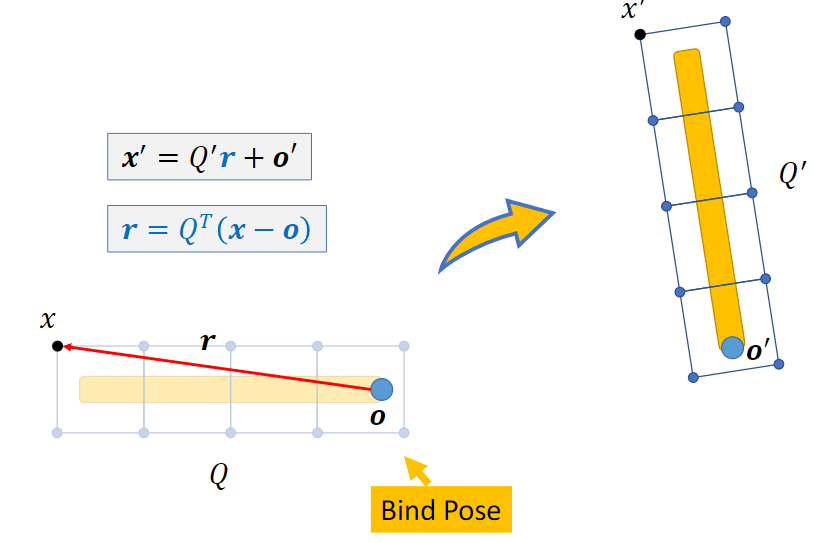
\includegraphics[width=0.618\linewidth]{pic/1057/Skinning Deformation}
    \caption{Skinning Deformation}
\end{figure}

Bind Pose: 在此姿态下计算 $\br$

对于多个骨骼, 在没旋转之前
\begin{align*}
    \br_1&= Q_1^\top (\bx-\bo_1)\\
    \br_2&=Q_2^\top (\bx-\bo_2)
\end{align*}
在旋转之后
\begin{align*}
    \bx'_1&=Q_1'\br_1 + \bo_1'\\
    \bx'_2&=Q_2'\br_2 + \bo_2'\\
    \bx' &= w_1\bx_1'+w_2\bx_2'
\end{align*}
但是旋转后一个点变成了两个点, 所以加个权重混合这两个点.

\begin{figure}[!htb]
    \centering
    \begin{subfigure}{0.618\linewidth}
        \centering
        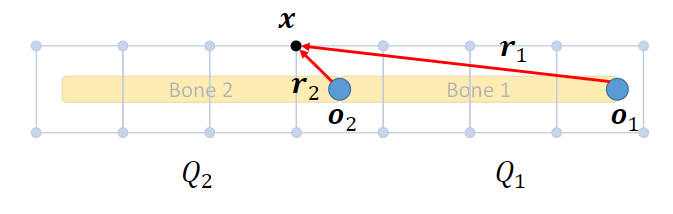
\includegraphics[width=\linewidth]{pic/1057/Skinning Deformation1}
        % \caption{Skinning Deformation1}
    \end{subfigure}
    \begin{subfigure}{0.618\linewidth}
        \centering
        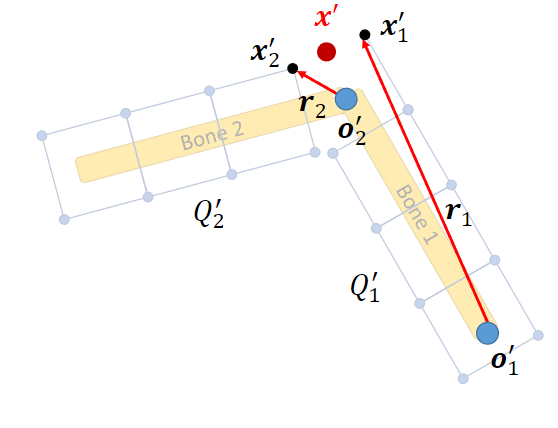
\includegraphics[width=\linewidth]{pic/1057/Skinning Deformation2}
        % \caption{}
    \end{subfigure}
    \caption{Skinning Deformation}
\end{figure}


\subsection{Linear Blend Skinning (LBS)}
线性混合蒙皮.
\begin{figure}[!htb]
    \centering
    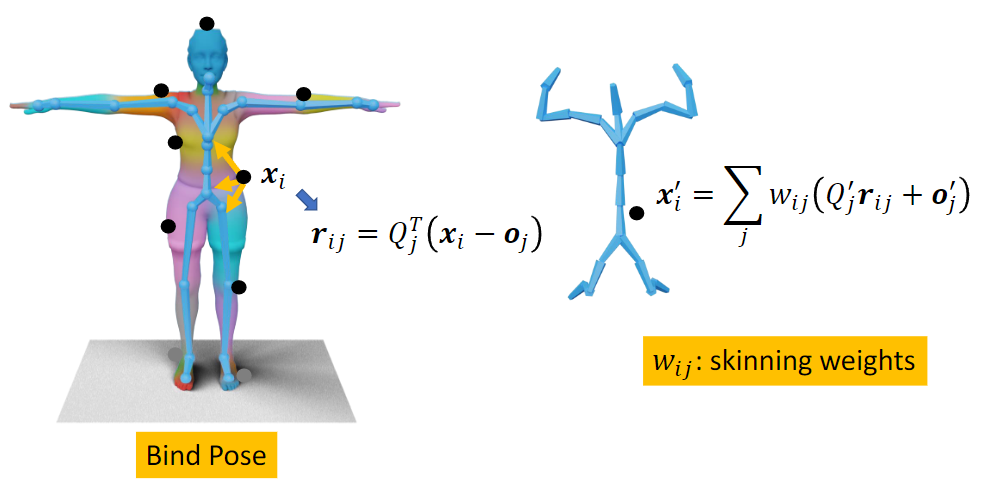
\includegraphics[width=0.88\linewidth]{pic/1057/Skinning}
    \caption{Skinning}
\end{figure}

\begin{itemize}
    \item 在 Bind pose / rest pose: 和 t-pose 不同, 其局部旋转不一定为 0
    \item 用 Skinning weights: 决定蒙皮质量
    \item 得到 Skinning transformation
\end{itemize}
这种方法高效, 且可并行, 游戏很常用. 

\begin{align*}
    \bx_i'&=\sum_{j=1}^m w_{ij}(Q_j'\br_{ij}+\bo_j')\\
    &=\sum_{j=1}^m w_{ij} \left(Q_j'Q_j^\top (\bx_i - \bo_j)+\bo_j'\right)\\
    &=\sum_{j=1}^m w_{ij} \left(Q_j'Q_j^\top \bx_i + \left(\bo_j' - Q_j'Q_j^\top  \bo_j \right)\right)\\
    &=\sum_{j=1}^m w_{ij}\left(R_j \bx_i + \bt_j\right)
\end{align*}

\begin{align*}
    \bx_i'&=\sum_{j=1}^m w_{ij}(R_j \bx_i + \bt_j)\\
    &=\sum_{j=1}^m w_{ij} R_j \bx_i + \sum_{j=1}^m w_{ij}\bt_j\\
    &=\left(\sum_{j=1}^m w_{ij} R_j \right)\bx_i + \sum_{j=1}^m w_{ij}\bt_j
\end{align*}



但是 $\left(\sum_{j=1}^m w_{ij} R_j \right)$ 是旋转矩阵的线性插值, 很容易出现插值后结果非线性矩阵的问题. 这种现象叫做 Candy-Wrapper Artifact (糖纸效应)

也不能换用其他可以插值的旋转表示, 因为其他旋转表示的旋转中心是坐标原点, 如果插值其和位移的配合是不好的.


\subsection{Dual Quaternion Skinning (DQS)}

% \subsubsection{Lie Group and Lie Algebra}
%TODO 摸了, 后面记得来补. P43, 43:15
% 逆天, 补一下李代数和李群吧 https://zhuanlan.zhihu.com/p/358455662
% https://murundb.github.io/kinematics/lie_group_and_lie_algebra/special_orthogonal_and_special_euclidean_groups/#definition

% \begin{definition}[General Linear Group]
%     Given a ring $R$ with identity, the general linear group $GL_n(R)$ is the group of $n\times n$ invertible matrices with elements in $R$.

%     The general linear group $GL_n(q)$ is the set of $n\times n$ matrices with entries in the field $F_q$ which have nonzero determinant.
% \end{definition}

% \begin{definition}[Projective General Linear Group]
%     The projective general linear group $PGL_n(q)$ is the group obtained from the general linear group $GL_n(q$) on factoring by the scalar matrices contained in that group.
% \end{definition}

% \begin{definition}[General Orthogonal Group]
%     The general orthogonal group $GO_n(q,F)$ is the subgroup of all elements of the projective general linear group that fix the particular nonsingular quadratic form $F$. The determinant of such an element is $ \pm 1$.
% \end{definition}

\begin{definition}[Special Orthogonal Group]
    The special orthogonal group $SO_n(q)$ is the subgroup of the elements of general orthogonal group $GO_n(q)$ with determinant $1$. 
    \begin{align*}
        SO(n)=\{ R\in \R^{n\times n} | R\times R^T = I | det (R)=1 \}
    \end{align*}

    $SO_3$ (often written $SO(3)$) is the rotation group for three-dimensional space.
\end{definition}

\begin{definition}[Special Euclidean Group]
    The group of rotations and translations.
    \begin{align*}
        SE(3)=\left\{ T=\begin{bmatrix}
            R & t \\
            0^T & 1
        \end{bmatrix} \in \R^{4\times 4} | R\in SO(3), t\in \R^3 \right\}
    \end{align*}
\end{definition}

\begin{figure}[!htb]
    \centering
    \includegraphics[width=0.88\linewidth]{pic/1057/lie_summary.png}
    \caption{Relationship between Lie group and Lie algebra}
\end{figure}

DQS(对偶四元数蒙皮) 用非线性变换来解决糖纸效应, 是 $SE(3)$ 内插值的近似. 

\subsubsection{Dual Number}
\begin{definition}[Dual Number]
    \begin{align*}
        x = a+b\epsilon
    \end{align*}
    where $\epsilon^2 = 0$
\end{definition}

\begin{itemize}
    \item Conjugate: 
    \begin{align*}
        \bar{x} = \overline{a+b\epsilon} = a-b\epsilon 
    \end{align*}
    \item Multiplication:
    \begin{align*}
        (a+b\epsilon)(c+d\epsilon) = ac + (ad+bc)\epsilon
    \end{align*}
\end{itemize}

\subsubsection{Dual Quaternion}
% A good note of dual-quaternion: https://faculty.sites.iastate.edu/jia/files/inline-files/dual-quaternion.pdf

\begin{definition}[Dual quaternion]
    \begin{align*}
        \hat{\bq} = \bq_0 + \epsilon \bq_\epsilon
    \end{align*}
    where $\epsilon^2=0$
\end{definition}

\begin{itemize}
    \item Scalar Multiplication:
    \begin{align*}
        s\hat{\bq} = s\bq_r + s \epsilon \bq_\epsilon 
    \end{align*}
    \item Addition: 
    \begin{align*}
        \hat{\bq}_1+\hat{\bq}_2 = \bq_{r_1} + \bq_{r_2} + \epsilon(\bq_{\epsilon_1} + \bq_{\epsilon_2})
    \end{align*}
    \item Multiplication: 
    \begin{align*}
        \hat{\bq}_1\hat{\bq}_2 = \bq_{r_1}\bq_{r_2}  + \epsilon (\bq_{r_1}\bq_{\epsilon_2}+\bq_{r_2}\bq_{\epsilon_1} )
    \end{align*}
    \item Conjugation:
    \begin{align*}
        \text{I: }\hat{\bq}^* & = \bq_0^* + \epsilon \bq_\epsilon^*\\
        \text{II: }\hat{\bq}^\circ & = \bq_0 - \epsilon \bq_\epsilon\\
        \text{III: }\hat{\bq}^\star & = \bq_0^* - \epsilon \bq_\epsilon^*\\
        &= (\hat{\bq}^*)^\circ =  (\hat{\bq}^\circ)^* \\
        (\hat{\bq}_1\hat{\bq}_2)^\times &= \hat{\bq}_2^\times\hat{\bq}_1^\times
    \end{align*}
    $\bq^*$ 代表四元数本身的共轭. I 是对四元数共轭,  II 是对对偶数共轭, III 是同时取共轭.
    \item Norm:
    \begin{align*}
        \norm{\hat{\bq}}= \sqrt{\hat{\bq}^*\hat{\bq}}=\norm{\bq_0}+ \frac{\epsilon(\bq_0\cdot \bq_\epsilon)}{\norm{\bq_0}}
    \end{align*}
    \item Unit dual quaternion:
    \begin{align*}
        \norm{\hat{\bq}} = 1
    \end{align*}
    where requires:
    \begin{align*}
        \norm{\bq_0} &= 1\\
        \bq_0 \cdot \bq_\epsilon&=0
    \end{align*}
\end{itemize}

\subsubsection{Dual Quaternion \texorpdfstring{$\iff$}.  Rigid Transformation}
类似四元数, 任何一个刚性变换 $T\in SE(3)$ 可转化为一个 单位对偶四元数
\begin{align*}
    T\bx &= R\bx + \bt\\
    T = [R|\bt] &\to \hat{\bq} = \bq_0+\epsilon\bq_\epsilon
\end{align*}
where
\begin{itemize}
    \item $\bq_0 = \br$ quaternion of $R$
    \item $\bq_\epsilon=\frac{1}{2}\bt \br$ pure quaternion $\bt = (0, t)$
\end{itemize}

Transform a vector $\bv$ using unit dual quaternion
\begin{align*}
    \hat{\bv}' = \hat{\bq}\hat{\bv}\hat{\bq}^*
\end{align*}
where $\hat{\bv} = 1+ \epsilon (0, \bv) = (1, 0, 0, 0) + \epsilon (0, v_x, v_y, v_z)$

$\hat{\bq}$ 和 $-\hat{\bq}$ 表示同一种变换. $\hat{\bm Q}$ 是 $SE(3)$ 的 double cover. 

\begin{figure}[!htb]
    \centering
    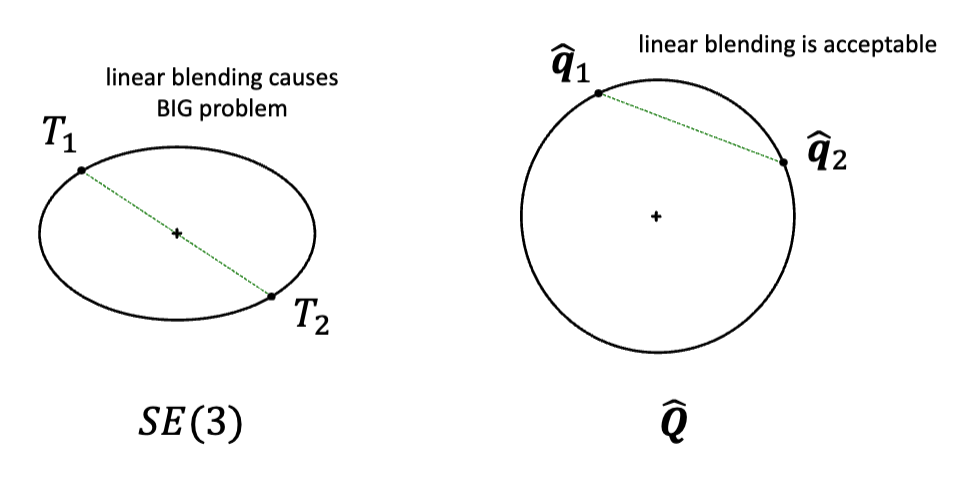
\includegraphics[width=0.88\linewidth]{pic/1057/Double Cover Visualized}
    \caption{Double Cover Visualized}
\end{figure}
对偶四元数求线性插值时, 通过取负号, 保证两个点的距离是小于半个圆周的(不过圆心)

\subsubsection{Dual-Quaternion Linear Blending (DLB)}
\begin{figure}[!htb]
    \centering
    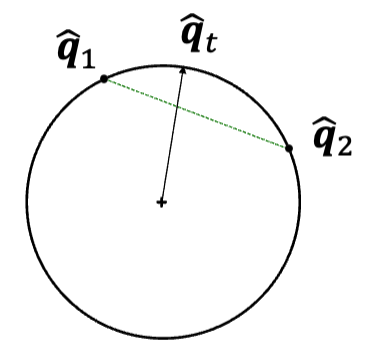
\includegraphics[width=0.42\linewidth]{pic/1057/DLB.png}
    \caption{DLB}
\end{figure}
所以求对偶四元数线性插值时, 可以直接插值后将结果投影到圆上, 这个操作始终是合理的. 

\begin{align*}
    \hat{\bq}_t &= (1-t)\hat{\bq}_0 + t\hat{\bq}_1\\
    \hat{\bq}_t &= \frac{(1-t)\hat{\bq}_0 + t\hat{\bq}_1}{\norm{(1-t)\hat{\bq}_0 + t\hat{\bq}_1}}
\end{align*}
但是插值角速度不是恒定的, 需要用特殊的插值方法保证插值角速度恒定.

\begin{figure}[!htb]
    \centering
    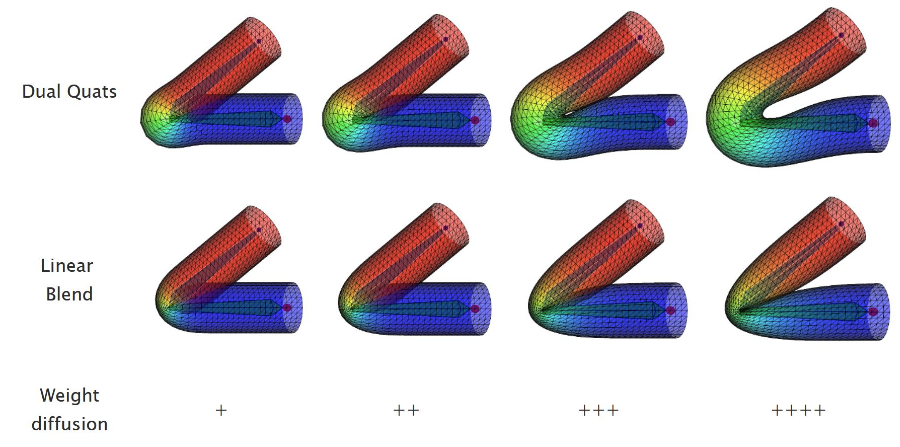
\includegraphics[width=0.618\linewidth]{pic/1057/Budging Artifact of DQS}
    \caption{Budging Artifact of DQS}
\end{figure}
DQS 的缺点: 胳膊肘会隆起.




\subsection{Blendshapes}
\subsubsection{Correct LBS}
在蒙皮上增加一个微小的修正项, 让结果更加光滑. 这个修正项应该与 $\bx$ 与 $\theta$ 相关
\begin{figure}[!htb]
    \centering
    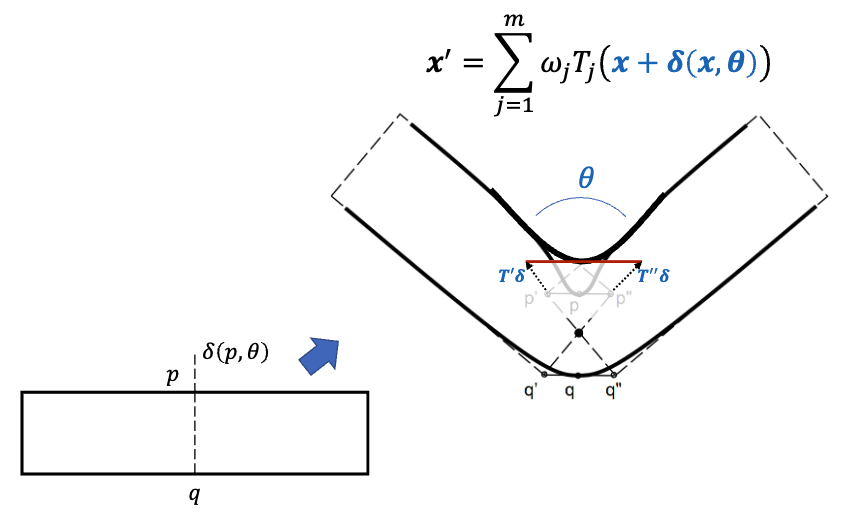
\includegraphics[width=0.618\linewidth]{pic/1057/Correct LBS}
    \caption{Correct LBS}
\end{figure}

\subsubsection{Example-based Shape Deformation}
\begin{figure}[!htb]
    \centering
    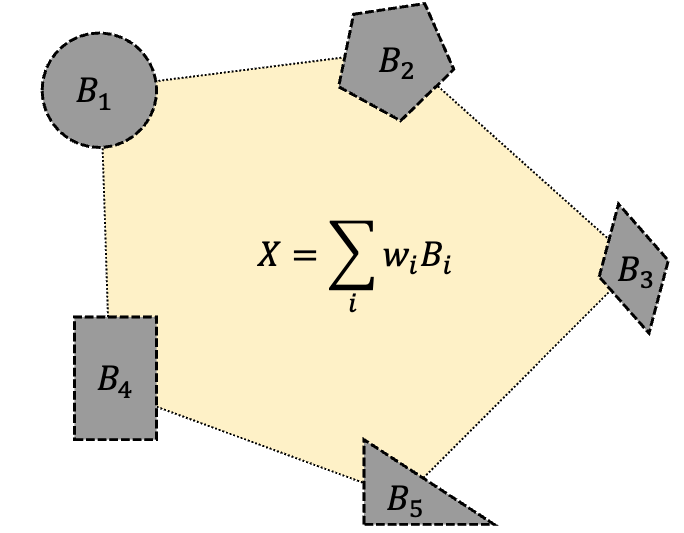
\includegraphics[width=0.618\linewidth]{pic/1057/Blendshapes}
    \caption{Blendshapes}
\end{figure}
定义一个空间, 对于其中的某个点可以计算出一个权重, 这个点所代表的形状就是根据权重进行插值后的结果. 这就是 Blendshapes / Blend Space

对于姿势, 就是给几个好的姿势, 有各自好的修正项, 新的姿势就是这几个姿势修正项的插值 . 

\subsubsection{Scattered Data Interpolation}
这就涉及到了高维空间的离散插值. 

以 Radial Basis Function (RBF) Interpolation 为例:
\begin{figure}[!htb]
    \centering
    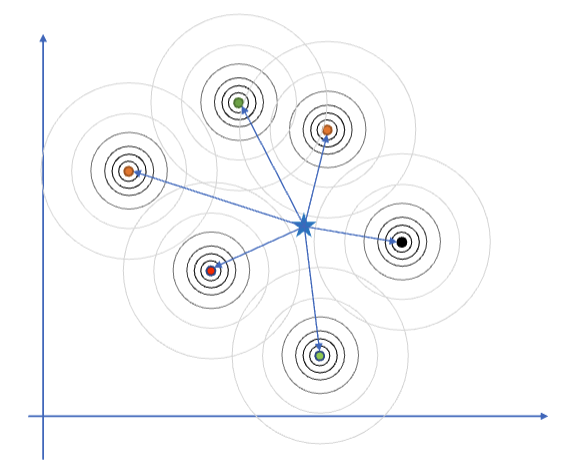
\includegraphics[width=0.618\linewidth]{pic/1057/RBF.png}
    \caption{RBF}
\end{figure}
\begin{align*}
    y=\sum_{i=1}^K w_i \varphi (\norm{x-x_i})
\end{align*}
但 $w_i$ 未知, 然后用待定系数法, 直接用已知的 $f(x_i)=y_i$ 求. 

对于 $\varphi$ 是预先定义好的, 有很多种. 比如 Gaussian $\varphi (r) = e^{-(\frac{r}{c})^2}$ 之类的. 
 
但是仍有很多问题, 不是完美的. 

\begin{figure}[!htb]
    \centering
    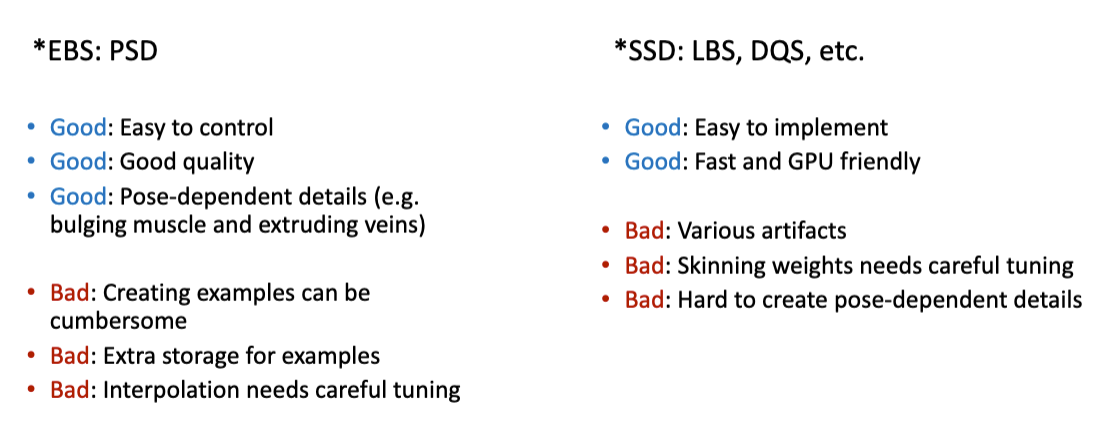
\includegraphics[width=0.88\linewidth]{pic/1057/Example-based Skinning (EBS) vs. Skeleton Subspace Deformation (SSD)}
    \caption{Example-based Skinning (EBS) vs. Skeleton Subspace Deformation (SSD)}
\end{figure}

\subsection{Examples}

\subsubsection{The SMPL model}
用 PCA 提取了人体数据的主成分. 

结果是主成分加了一个修正项, 修正项是用了个高维线性拟合. 

\begin{align*}
    T(\beta, \theta) = \bar{T} + \sum_{m=1}^{|\beta|}\beta_m S_n + \sum_{n=1}^{|\theta|}\theta_np_n
\end{align*}


\subsubsection{Facial Animation}
\begin{figure}[!htb]
    \centering
    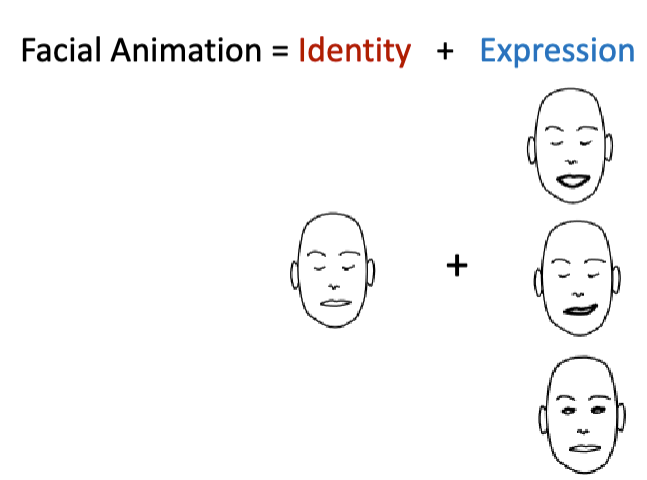
\includegraphics[width=0.618\linewidth]{pic/1057/Facial Animation}
    \caption{Facial Animation}
\end{figure}

\begin{align*}
    X= X_0 + \sum_i \beta_i B_i^{ID} + \sum_j \theta_j B_j^{Exp}
\end{align*}